\chapter{Estado del arte en técnicas de fusión sensorial}
\label{cha:Estado del arte en técnicas de fusión sensorial}

\begin{FraseCelebre}
  \begin{Frase}
    Texto.
  \end{Frase}
  \begin{Fuente}
    Autor texto
  \end{Fuente}
\end{FraseCelebre}

\noindent
Antes de presentar la propuesta de trabajo sobre la que se basa este TFM, es necesario comprender múltiples técnicas pertenecientes al estado del arte que han sido estudiadas de forma previa a la definición de este trabajo. Esto es debido a que múltiples conceptos que se presentan es estos modelos se volverán a utilizar a lo largo del trabajo por lo que es recomendable comprenderlos para entender de mejor manera lo que se ha realizado. Más adelante se explicará cómo dos de los modelos a continuación presentados han influenciado en gran medida en las decisiones tomadas respecto al diseño del modelo de detección que se ha realizado.

\section{MV3D}
\label{sec:MV3D}

El modelo \ac{MV3D} \cite{MV3D} se basa en una representación multivista de la nube de puntos 3D y una imagen. Primero genera propuestas de objetos 3D a partir del mapa en vista de pájaro o \ac{BEV}, y fusiona las características de las múltiples vistas mediante una representación basada en regiones. Las características fusionadas se utilizan para la clasificación de categorías y la regresión de cajas o bounding boxes 3D.

Analizando la entrada de la red, se observa el uso de dos sistemas de análisis basados en la nube de puntos del \ac{LiDAR}, junto con la imagen frontal de la cámara del vehículo. Por una parte, la nube de puntos se representa en \ac{BEV} como múltiples matrices 2D, en las que se representan diferentes mapas de altura del entorno, un mapa de densidad en relación a la cantidad de puntos, y un mapa de intensidad según el valor de reflectividad de la nube de puntos en cada zona. La otra representación de la nube de puntos consiste en su transformación al eje de la cámara, para su posterior codificación en función de la altura, la distancia y la intensidad.

Entrando en detalles del modelo, primero se comienza procesando la nube de puntos en \ac{BEV} mediante un modelo convolucional (los cuales se explicarán más adelante en el capítulo \ref{sec:Convolutional Neural Networks}), tras el cual se obtienen unas primeras propuestas de detecciones 3D, las cuales son utilizadas para su transformación a vista de pájaro, como detecciones 2D frontales.

\begin{figure}[H]
    \centering
    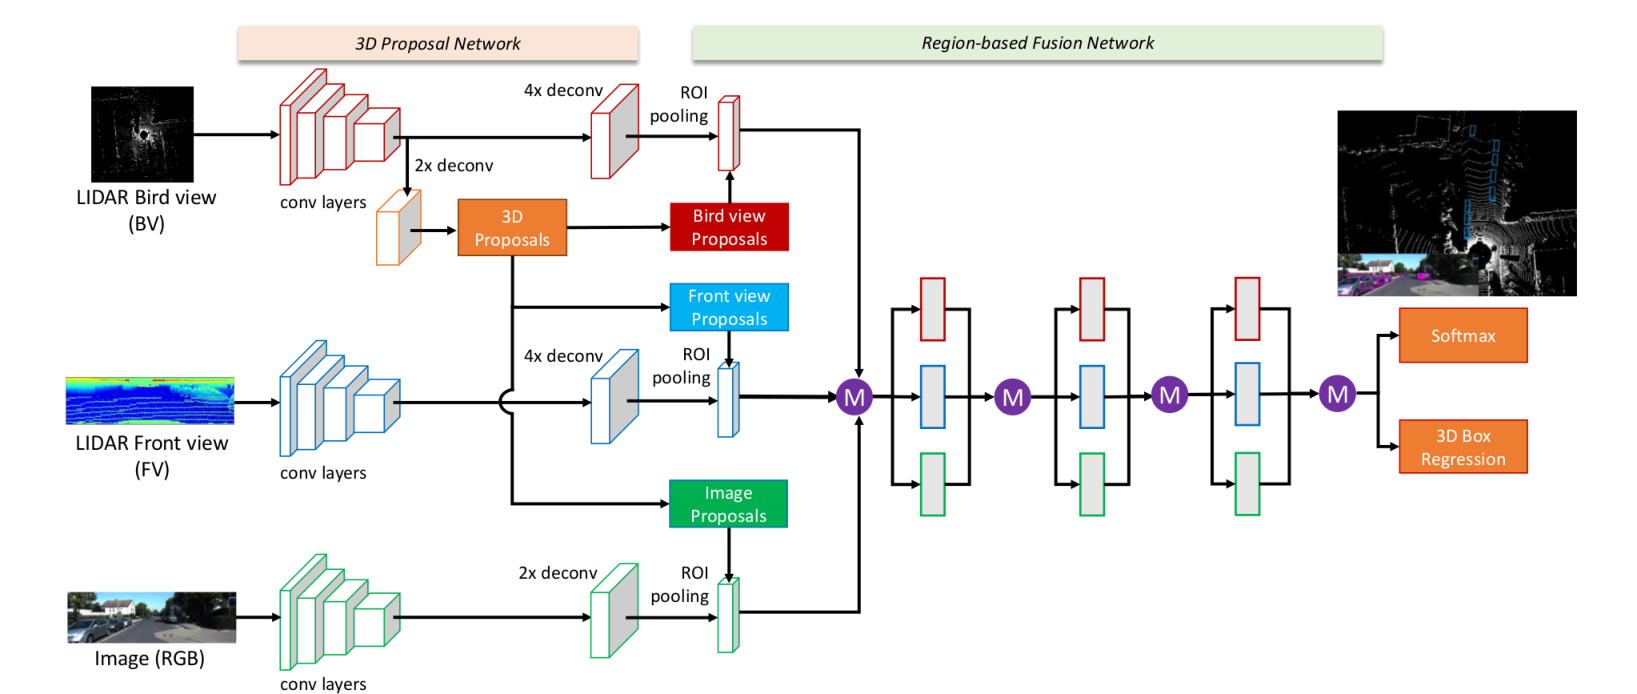
\includegraphics[width=0.8\textwidth]{Book/figures/2_estado_arte/MV3D.png}
    \caption{Arquitectura del modelo MV3D.}
    \label{fig:Arquitectura del modelo MV3D.}
\end{figure}

Mediante la aplicación de modelos convolucionales sobre todas las entradas del modelo, y la fusión con las detecciones inicialmente obtenidas de forma frontal y en vista de pájaro en función de cada una de las entradas, se obtienen multitud de detecciones, por lo que se aplica el algoritmo \ac{NMS} para eliminar las detecciones que se superponen. Como método de unificar las diferentes ramas del flujo de trabajo se analizan las regiones de interés o \ac{RoI}, donde se encuentran las detecciones para obtener vectores de características de las mismas dimensiones.

Hasta este punto, las características de las 3 fuentes de entrada no han sido tratadas de forma conjunta, por lo que comienza la fase de Deep Fusion, donde se fusionan las características de las diferentes vistas. Para ello, tras concatenar los vectores de características de las distintas fuentes, estas son analizadas con múltiples modelos neuronales. Tras la repetición de este modelo de Deep Fusion 3 veces, se obtienen las clases de los objetos junto con las detecciones 3D correspondientes.

La vista general del modelo se puede observar en la Figura \ref{fig:Arquitectura del modelo MV3D.}, la cual muestra cada una de las fases explicadas. La importancia en la explicación de este modelo radica en la comprensión de la gran posibilidad de formas de entrada en una red neuronal de los datos del \ac{LiDAR} junto con el uso de imágenes además de la comprensión de múltiples términos como: \ac{NMS}, \ac{RoI} o Deep Fusion; ya que son ampliamente utilizados en el campo de la visión artificial. En cuanto a la puesta en producción de este modelo, se descarta debido a la velocidad de inferencia de 0,36 segundos en una tarjeta gráfica NVIDIA GeForce Titan X.

\section{Frustum PointNets}
\label{sec:Frustum PointNets}

El modelo Frustum PointNets \cite{Frustum_PointNets} trata de obtener detecciones 3D de los objetos del entorno a partir de una imagen con información RGB-D, siendo esa última 'D' un parámetro de distancia definido por la proyección de la nube de puntos del \ac{LiDAR} sobre la imagen. A partir de este tratamiento de los datos presentado en este paper, se trasforma esta imagen de entrada en un tronco de pirámide 3D o frustum que representa el espacio en el que se encuentra el objeto a detectar tridimensionalmente.

La cantidad de información producida por parte de los sensores 3D utilizados es menor a la que provee una imagen RGB, por ello se utiliza de forma principal las imágenes producidas por la cámara. Conociendo la matriz de parámetros intrínsecos de la cámara junto con la posición relativa al \ac{LiDAR}, se puede transformar la nube de puntos para proyectarse sobre el plano de la cámara, el cual es una de la entradas de este modelo. A partir de un modelo convolucional (sin concretar) del que obtenga el tipo de los objetos junto con las regiones de interés 2D, las cuales son utilizadas para el filtrado de la nube de puntos.

A partir de las regiones de interés 2D en la nube de puntos proyectada a la imagen, se transforma de nuevo en una nube de puntos 3D en la que únicamente se tienen los puntos de la región de interés obtenida previamente. De esta manera se puede introducir esta nube de puntos en un modelo como PointNet \cite{PointNet} (el cual se explicará más en profundidad en el Capítulo \ref{sec:PointNet}) para obtener junto con el tipo del objeto de la región, cada uno de los puntos de la región de interés segmentados para discernir los puntos que inciden en el objeto a detectar.

\begin{figure}[H]
    \centering
    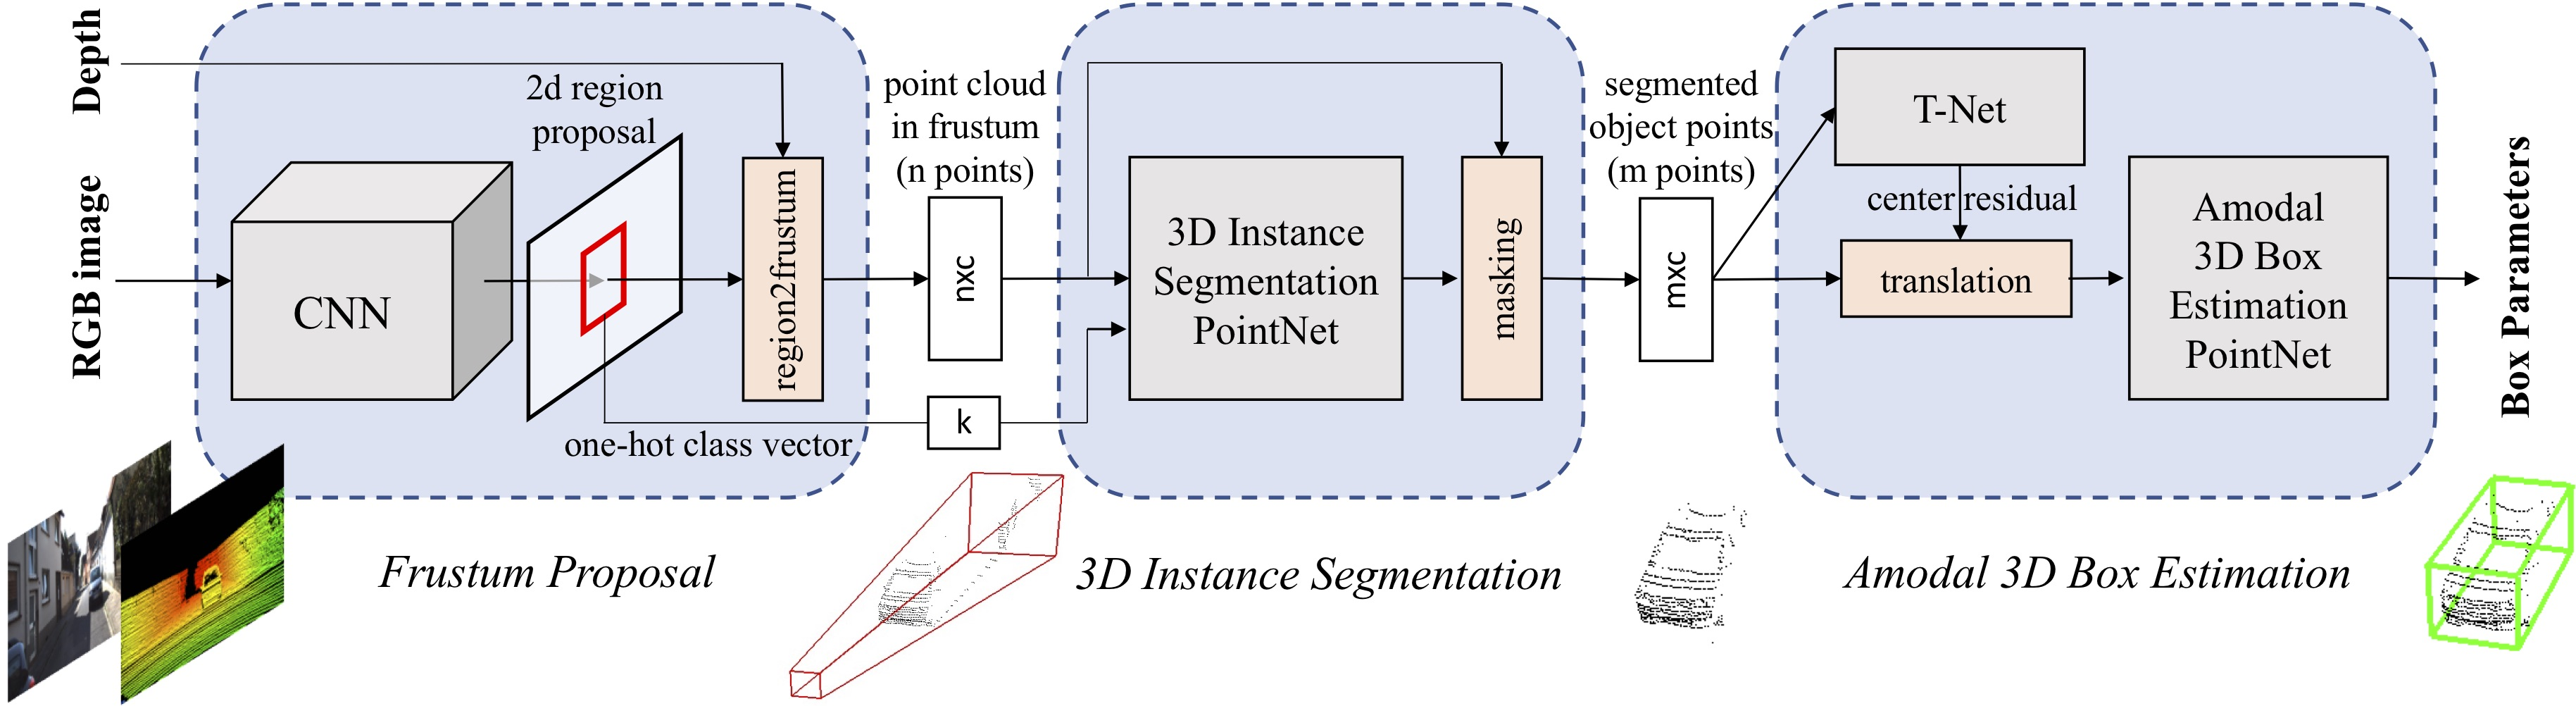
\includegraphics[width=1\textwidth]{Book/figures/2_estado_arte/frustum_pointnets.png}
    \caption{Arquitectura del modelo Frustum PointNets.}
    \label{fig:Arquitectura del modelo Frustum PointNets.}
\end{figure}

Con la nube de puntos segmentada, se procede a eliminar todos los puntos que no inciden en el vehículo. Para obtener una entrada más sencilla con la que obtener la bounding box 3D del objeto analizado, se crea una pequeña red en la que se infiere el centro del objeto, para posteriormente mover dicho objeto al origen del eje de coordenadas con el que se trabaja. Tras este último paso, se procede a obtener las bounding boxes 3D finales mediante un acercamiento similar al procesamiento realizado por PointNet. De esta manera se obtiene tanto el tamaño como la rotación del objeto de interés.

Este modelo aun teniendo múltiples pasos intermedios hasta conseguir las detecciones finales como se ha explicado y se ve en la Figura \ref{fig:Arquitectura del modelo Frustum PointNets.}, consigue unos resultados muy competentes en un bajo tiempo de inferencia sobre una NVIDIA GTX 1080 de 88 ms utilizando el modelo que se basa en PointNet en vez de PointNet++ \cite{PointNet++}. La idea de trabajar con frustums, es un tipo de procesamiento que se utilizará en el modelo diseñado en este trabajo, por lo que este paper tiene una gran influencia en el trabajo a realizar.

\section{PointPainting}
\label{sec:PointPainting}

La arquitectura PointPainting \cite{PointPainting} trata de solucionar el problema de la detección de objetos 3D mediante el uso de nubes de puntos e imágenes. Para ello presenta un sistema de detección de objetos basado en 3 etapas principales: una primera etapa de segmentación semántica, una fase de pintado de la nube de puntos y una última etapa de detección de los objetos 3D.

En la primera fase se utiliza la imagen del entrada proporcionada por la cámara para realizar la segmentación semántica. Dicho proceso de segmentación semántica consiste en la creación un máscara, en la cual se indique a nivel de píxel las regiones que pertenecen o no a las clases que se quieren detectar, como son: coches, peatones o ciclistas. Para ello se utiliza el modelo DeepLabv3+ \cite{DeepLabv3+} para la obtención de la imagen de entrada segmentada, realizando esto tras el entrenamiento de este modelo sobre el dataset KITTI.

La fase de pintado de la nube de puntos requiere del uso de la matriz intrínseca de la cámara y de las matrices de traslación y rotación entre la cámara y el \ac{LiDAR}. Esto es así debido al proceso de adición de una nueva dimensión en la nube de puntos, lo cual es producido al transformar la máscara que identifica las regiones en las que se encuentra cada clase, sobre la nube de puntos. En el caso del uso sobre el dataset KITTI se utilizan únicamente 4 clases para la nueva dimensión como son: coche, peatón, ciclista y resto. Gracias a este proceso es mucho más sencillo discernir sobre la nube de puntos donde se encuentran todos los objetos y simplificar el proceso de obtención de las bounding boxes 3D.

En la tercera y última fase de detección se utiliza el modelo PointPillars \cite{PointPillars} (el cual se presentará más adelante en el Capítulo \ref{sec:PointPillars}) para producir las detecciones 3D finales, que gracias al proceso de aporte de información a la nube de puntos al introducir el dato de que puntos inciden en los objetos de interés, puede producir unas mejores detecciones. Este mismo proceso se ha probado y funciona perfectamente sobre cualquier modelo de detección 3D utilizando \ac{LiDAR}, solo que es necesaria la adición de una dimensión en la entrada del modelo a utilizar en comparativa al uso de una nube de puntos tradicional.

\begin{figure}[H]
    \centering
    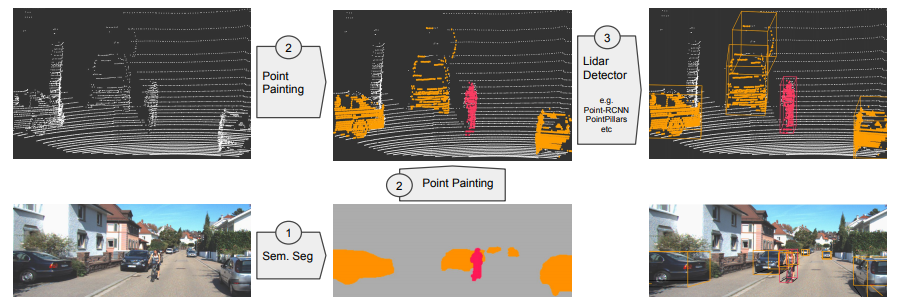
\includegraphics[width=1\textwidth]{Book/figures/2_estado_arte/painted_pointpillars.png}
    \caption{Pasos del modelo PointPainting.}
    \label{fig:Pasos del modelo PointPainting.}
\end{figure}

El modelo PointPainting se compone de etapas muy claras y sencillas por lo que es muy fácil su implementación en un pipeline de visión, como se ve en la Figura \ref{fig:Pasos del modelo PointPainting.}. De forma adicional consigue resultados muy buenos en los datasets de KITTI y nuScenes en las tareas de detección 3D y detección 2D en \ac{BEV}. En cuanto al tiempo de ejecución, no se conoce exactamente el tiempo de inferencia completo ya que en el paper solo se estudia el tiempo de pintado de la nube de puntos y la fase de detección, el cual es muy similar al tiempo de ejecución del modelo utilizado para obtener las detecciones. Analizando el ranking de nuScenes se encuentra que en el test online de ese dataset se obtiene una velocidad de inferencia de 27,6Hz en comparación con PointPillars que tiene una velocidad de 61,2 Hz sobre el mismo hardware, por lo que se podría implementar para su uso en tiempo real.